\scalebox{0.6}{
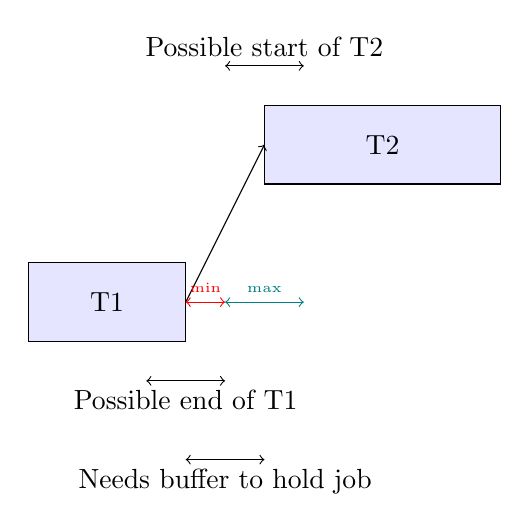
\begin{tikzpicture}
\draw[fill=blue!10,draw=black] (0,0) rectangle node {T1} (2,1);
\draw[fill=blue!10,draw=black] (3,2) rectangle node {T2} (6,3);
\draw[->] (2,0.5) -- (3,2.5);
\draw[<->,red] (2,0.5) -- node[above] {\tiny min} (2.5,0.5);
\draw[<->,teal] (2.5,0.5) -- node[above] {\tiny max} (3.5,0.5);
\draw[<->] (2.5,3.5) -- node[above] {Possible start of T2} (3.5,3.5);
\draw[<->] (1.5,-0.5) -- node[below] {Possible end of T1} (2.5,-0.5);
\draw[<->] (2,-1.5) -- node[below] {Needs buffer to hold job} (3,-1.5);
\end{tikzpicture}
}